\section{PDE2: Navier--Stokes Equations with Spalart--Allmaras Closure}
\label{sec:NSE-SA}

\renewcommand{\thefigure}{D.\arabic{figure}}  % Number figures as A.1, A.2, ...
\renewcommand{\thetable}{D.\arabic{table}}  % Number tables as A.1, A.2, ...


\subsection*{Problem setup}
We simulate two-dimensional incompressible flows in the unit square domain \( \mathcal{X} = [0, 1] \times [0, 1] \) over the time interval \( t \in [0, T] \) with \( T = 25 \). The governing equations are expressed in vorticity--stream function form, coupled with the one-equation Spalart--Allmaras (S-A) turbulence model. Let \( \mathbf{x} = (x_1, x_2) \in \mathcal{X} \). The system reads:
\begin{align}
\nabla^2 \Psi &= -\Omega, \label{eq:streamfunction} \\[4pt]
\frac{\partial \Omega}{\partial t}
+ \frac{\partial \Psi}{\partial x_2} \frac{\partial \Omega}{\partial x_1}
- \frac{\partial \Psi}{\partial x_1} \frac{\partial \Omega}{\partial x_2}
&= \nabla \cdot \bigl[ (\nu + \nu_t) \nabla \Omega \bigr] + f(\mathbf{x}; \alpha, \beta), \label{eq:vorticity} \\[6pt]
\frac{\partial \tilde{\nu}}{\partial t}
+ \frac{\partial \Psi}{\partial x_2} \frac{\partial \tilde{\nu}}{\partial x_1}
- \frac{\partial \Psi}{\partial x_1} \frac{\partial \tilde{\nu}}{\partial x_2}
&= c_{b1} \tilde{S} \tilde{\nu}
+ \frac{1}{\sigma} \left[ \nabla \cdot \bigl( (\nu + \tilde{\nu}) \nabla \tilde{\nu} \bigr) + c_{b2} (\nabla \tilde{\nu})^2 \right]
- c_{w1} f_w \left( \frac{\tilde{\nu}}{d} \right)^2, \label{eq:SA}
\end{align}
where $\Psi$ denotes the stream function, $\Omega$ the vorticity, and the molecular viscosity is taken as $\nu \in [0.001,\,0.002]$, which corresponds to Reynolds numbers in the range $500$--$1000$. The turbulent eddy viscosity is modeled as $\nu_t = \tilde{\nu}\, f_{v1}$.
\[
f_{v1} = \frac{\chi^3}{\chi^3 + c_{v1}^3}, \quad \chi = \frac{\tilde{\nu}}{\nu}.
\]
The term \( f(\mathbf{x}; \alpha, \beta) \) is a parametric body force, and \( d \) is the distance to the nearest wall.

Physical boundary conditions are no-slip walls (\( \mathbf{u} = 0 \)), implying \( \Psi = 0 \) and \( \partial \Psi / \partial n = 0 \) on \( \partial \mathcal{X} \). Vorticity vanishes on walls via the initial mask \( m(x_1, x_2) = \sin(\pi x_1) \sin(\pi x_2) \).

The numerical solver uses zero wall boundary conditions in both directions for its finite difference discretization and fast Poisson solving. Physical wall conditions are enforced weakly through:
\begin{itemize}
    \item Initial vorticity masking to ensure \( \Omega_0 = 0 \) on wall-adjacent cells,
    \item Spectral projection of \( \Psi \) after each Poisson solve to satisfy \( \Psi = 0 \) on \( \partial \mathcal{X} \),
    \item Thom’s formula at each time step to enforce \( \mathbf{u} = 0 \) on walls.
\end{itemize}

The forward simulation uses a uniform fine grid of resolution \( 64 \times 64 \). The initial modified eddy viscosity is sampled from a Gaussian random field (GRF):
\[
\tilde{\nu}_0(\mathbf{x}) \sim \text{GRF}\bigl(p_{\min} = -2.5 \times 10^{-4},\; p_{\max} = 2.5 \times 10^{-4},\; \sigma = 1,\; \mathcal{X}\bigr).
\]

The initial vorticity \( \Omega_0 \) is generated on a coarse grid of resolution \( N_c \times N_c \), where \( N_c = 2^n \) and \( n \in \{2, 3, 4, 5, 6\} \) (corresponding to \( N_c \times N_c \in \{4\times4, 8\times8, 16\times16, 32\times32, 64\times64\} \)). For a given \( n \), the coarse field is
\[
\Omega_0^c(\mathbf{x}) = m(x_1, x_2) \cdot \text{GRF}\bigl(p_{\min} = -2.5,\; p_{\max} = 2.5,\; \sigma = 2,\; \mathcal{X}_c^n\bigr),
\]
upsampled to \( 64 \times 64 \) via pixel-wise repetition by factor \( 2^{6-n} \). This ensures zero vorticity on wall-adjacent fine-grid cells and introduces multiscale initial perturbations.

The forcing is
\[
f(\mathbf{x}; \alpha, \beta) = 0.1 \left[ \sin\!\bigl(\alpha (x_1 + x_2)\bigr) + \cos\!\bigl(\beta (x_1 + x_2)\bigr) \right],
\]
with \( \alpha, \beta \in [0, 3\pi] \) sampled uniformly.

\subsection*{Numerical Solver for the Turbulent Navier--Stokes Equations}

The system is recast as an ODE:
\[
\frac{d\mathbf{U}}{dt} = \text{RHS}(\mathbf{x}, t; p), \quad \mathbf{U} = [\Omega, \tilde{\nu}],
\]
with \( \Psi \) recovered via a fast Poisson solver (e.g., a Sine Transform) under zero wall computational boundary conditions. Spatial discretization uses second-order central finite differences on uniform grids. Time integration uses the Fourth Order Runge-Kutta solver from \texttt{torchdiffeq}, storing solutions at \( \Delta t = 0.1 \) over \( [0, 25.0] \), yielding \( n_t = 250 \) snapshots. The solver is fully differentiable, enabling adjoint-based gradients with respect to \( \Omega_0 \) and the forcing term.





\subsection*{Neural Operator Learning for the Turbulent Navier--Stokes Equations}

We employ neural operator learning to tackle the turbulent Navier--Stokes equations with the Spalart--Allmaras model over a spatial domain $\mathcal{X}$ and time $t \in [0, 25.0]$, discretized into $n_t$ snapshots (here, $n_t=250$ at $\Delta t=0.1\,\mathrm{s}$). The parametric, spatially varying forcing $f(\mathbf{x}; \alpha,\beta)$ acts as the parameter field $p(\mathbf{x})$ within the input function $a(\mathbf{x}, t, p)\in\mathcal{U}$. The solution state is $u(\mathbf{x}, t, p) = [\Psi(\mathbf{x}, t),\, \Omega(\mathbf{x}, t),\, \tilde{\nu}(\mathbf{x}, t)]$.

\paragraph{(I) Sequential multi-step forecasting (context $\rightarrow$ full-horizon prediction).}
We train a neural operator $\mathcal{G}_\theta$ within the SC-NO framework that consumes a short context of the trajectory together with the forcing field and predicts the remainder of the sequence in one shot. Concretely, the input consists of the initial segment of the solution field \( u(\mathbf{x}, t, p) \) over \( t \in [0, t_u] \) and the parameter field \( p(\mathbf{x}) = f(\mathbf{x}; \alpha, \beta) \):
\[
\mathcal{G}_\theta:\; \big(u(\mathbf{x}, t, p)\big)_{t \in [0, t_u]},\, p(\mathbf{x})\;\longrightarrow\; u(\mathbf{x}, t, p),
\quad (\mathbf{x}, t) \in \mathcal{X} \times [t_u,\,25.0].
\]
The training loss aggregates the state error over all predicted times together with a sensitivity regularizer. This regime corresponds to the “sequential prediction” setting used in the main text.



Additionally, to evaluate the model’s sensitivity to spatial resolution, we construct a family of simulations with multiresolution initial vorticity fields. Specifically, the base vorticity field \( \Omega_0^c(\mathbf{x}) \) is generated on coarse grids \( \mathcal{X}_c^n \) with \( N_c = 2^n \), \( n \in \{2,3,4,5,6\} \), and then upsampled to the working grid \( \mathcal{X} \) for training. Each resolution level thus defines a distinct realization of the input sequence \( \big(u(\mathbf{x}, t, p)\big)_{t \in [0, t_u]} \), differing only in the spatial smoothness and detail of the initial vorticity \( \Omega_0(\mathbf{x}) \). The operator learns the mapping  
\[
\mathcal{G}_\theta:\; \big(u(\mathbf{x}, t, p)\big)_{t \in [0, t_u]},\, p(\mathbf{x})\;\longrightarrow\; u(\mathbf{x}, t, p),
\quad (\mathbf{x}, t) \in \mathcal{X} \times [t_u,\,25.0],
\]
allowing us to systematically assess how prediction accuracy and learned sensitivities vary across different resolutions of the initial vorticity field.




\paragraph{(II) One-step transition with autoregressive rollout (rollout model).}  
In this regime, we train a \emph{transition operator} that advances the state by a single time step given the current state and the forcing field. During training, the operator is supervised on consecutive snapshot pairs using teacher forcing. Specifically, it learns the mapping
\[
\mathcal{F}_\theta:\; \big(u(\cdot,t,p),\, p(\mathbf{x})\big)\;\longrightarrow\; u(\cdot,t+\Delta t,p),
\]
with training pairs $\big(u(\cdot,t,p),\, u(\cdot,t+\Delta t,p)\big)$ drawn from the first 125 snapshots, corresponding to $t \in [0,12.5]$\,s. To improve robustness, the predicted states used during training are perturbed with controlled noise before being fed back as inputs, preventing the model from overfitting to perfectly clean trajectories.  

At inference time, the learned operator is applied recursively in an autoregressive manner to generate full trajectories. Starting from the initial condition $u(\cdot,0,p)$, we roll the model forward for 250 steps to cover the entire horizon $[0,25.0]$\,s:  
\[
\hat{u}(\cdot,t+\Delta t,p)=\mathcal{F}_\theta\!\big(\hat{u}(\cdot,t,p),\,p\big), \quad t=0,\Delta t,2\Delta t,\ldots,25.0-\Delta t.
\]
This formulation explicitly probes long-horizon stability and error accumulation: the model is trained only on short-range one-step transitions ($0$–$12.5$\,s) but evaluated on the full $0$–$25$\,s trajectory (250 snapshots).  

\subsection*{Adjoint-Based Sensitivity Computation for the Turbulent Navier--Stokes Equations}
\label{sec:adjoint_nse}

To compute sensitivities of the final-time vorticity field $\Omega(\mathbf{x}, T)$ with respect to the initial vorticity $\Omega_0(\mathbf{x})$ and the forcing $f(\mathbf{x}, t; \alpha, \beta)$, we derive the continuous adjoint system. The adjoint method is a powerful technique for efficiently computing the sensitivity of a scalar objective functional, $J$, to a large number of input parameters or fields (such as initial conditions $\Omega_0$ or forcing $f$). Its primary advantage is that the computational cost of obtaining the gradient is \textbf{independent} of the number of input parameters. The method relies on constructing a Lagrangian, $\mathcal{L}$, which augments the objective functional with the governing PDEs, enforced as constraints via Lagrange multipliers (the adjoint variables, e.g., $\lambda_\Omega, \lambda_{\tilde{\nu}}$). By requiring the first variation of the Lagrangian ($\delta\mathcal{L}$) to be zero with respect to the state variables, a new set of linear PDEs—the \textbf{adjoint equations}—is derived.

These adjoint equations are solved \textbf{backward in time}, starting from a terminal condition derived from the objective functional at $t=T$. The resulting adjoint field, $\lambda(\mathbf{x}, 0)$, at the initial time $t=0$ (or integrated over time for forcing) provides the exact functional derivative (gradient) of $J$ with respect to the parameters. This allows the gradient for all parameters to be computed from just one forward solve of the primal equations and one backward solve of the adjoint equations.

\subsubsection*{Cost Functional}

The cost functional is the integrated final vorticity:
\begin{equation}
J = \int_{\mathcal{X}} \Omega(\mathbf{x}, T) \, d\mathbf{x}.
\end{equation}

\subsubsection*{Lagrangian Formulation}

The Lagrangian is
\begin{align}
\mathcal{L} &= \int_{\mathcal{X}} \Omega(T) \, d\mathbf{x} \notag \\[4pt]
&\quad + \int_0^T \int_{\mathcal{X}} \lambda_{\Omega} \left[
\frac{\partial \Omega}{\partial t}
+ (\mathbf{u} \cdot \nabla) \Omega
- \nabla \cdot \bigl( \nu_{\text{eff}}(\tilde{\nu}) \nabla \Omega \bigr)
- f
\right] d\mathbf{x} \, dt \notag \\[4pt]
&\quad + \int_0^T \int_{\mathcal{X}} \lambda_{\tilde{\nu}} \left[
\frac{\partial \tilde{\nu}}{\partial t}
+ (\mathbf{u} \cdot \nabla) \tilde{\nu}
- \frac{1}{\sigma} \nabla \cdot \bigl( (\nu + \tilde{\nu}) \nabla \tilde{\nu} \bigr)
- \frac{c_{b2}}{\sigma} (\nabla \tilde{\nu})^2
- R(\Omega, \tilde{\nu})
\right] d\mathbf{x} \, dt \notag \\[4pt]
&\quad + \int_0^T \int_{\mathcal{X}} \lambda_{\Psi} \left[
\nabla^2 \Psi + \Omega
\right] d\mathbf{x} \, dt,
\end{align}
where $\mathbf{u} = \nabla^\perp \Psi$, $\nu_{\text{eff}}(\tilde{\nu}) = \nu + \tilde{\nu} f_{v1}(\tilde{\nu})$, and
\[
R(\Omega, \tilde{\nu}) = c_{b1} \tilde{S} \tilde{\nu} - c_{w1} f_w \left( \frac{\tilde{\nu}}{d} \right)^2.
\]

\subsubsection*{Adjoint Equations}

The first variation $\delta \mathcal{L} = 0$ with respect to $(\Psi, \Omega, \tilde{\nu})$ yields the adjoint system. Integration by parts in space and time is performed. Boundary terms are eliminated using primal wall conditions.

\textbf{Adjoint Poisson Equation} (from $\delta \Psi$):
\begin{equation}
\nabla^2 \lambda_{\Psi}
= -\nabla^\perp \cdot (\lambda_{\Omega} \nabla \Omega)
  -\nabla^\perp \cdot (\lambda_{\tilde{\nu}} \nabla \tilde{\nu}).
\end{equation}

\textbf{Adjoint Vorticity Equation} (from $\delta \Omega$):
\begin{equation}
-\frac{\partial \lambda_{\Omega}}{\partial t}
= \mathbf{u} \cdot \nabla \lambda_{\Omega}
  + \nabla \cdot \bigl( \nu_{\text{eff}} \nabla \lambda_{\Omega} \bigr)
  + \lambda_{\Psi}
  + \lambda_{\tilde{\nu}} \frac{\partial R}{\partial \Omega},
\end{equation}
with
\[
\frac{\partial R}{\partial \Omega}
= c_{b1} \tilde{\nu} \frac{\partial \tilde{S}}{\partial \Omega},
\qquad
\frac{\partial \tilde{S}}{\partial \Omega}
= \operatorname{sgn}(\Omega)
\quad \text{(regularized as $\tanh(k \Omega)$ in practice)}.
\]

\textbf{Adjoint Spalart--Allmaras Equation} (from $\delta \tilde{\nu}$):
\begin{equation}
-\frac{\partial \lambda_{\tilde{\nu}}}{\partial t}
= \mathbf{u} \cdot \nabla \lambda_{\tilde{\nu}}
  + \frac{1}{\sigma} \nabla \cdot \bigl( (\nu + \tilde{\nu}) \nabla \lambda_{\tilde{\nu}} \bigr)
  - \nabla \cdot \left( \frac{2 c_{b2}}{\sigma} \lambda_{\tilde{\nu}} \nabla \tilde{\nu} \right)
  + \lambda_{\tilde{\nu}} \frac{\partial R}{\partial \tilde{\nu}}
  - \frac{\partial \nu_{\text{eff}}}{\partial \tilde{\nu}} (\nabla \lambda_{\Omega} \cdot \nabla \Omega).
\end{equation}

\subsubsection*{Adjoint Terminal and Boundary Conditions}

\textbf{Terminal conditions} (at $t = T$):
\begin{align}
\lambda_{\Omega}(\mathbf{x}, T) &= -1, \\
\lambda_{\tilde{\nu}}(\mathbf{x}, T) &= 0.
\end{align}

\textbf{Boundary conditions} (on $\partial \mathcal{X}$, $0 \leq t < T$):
\begin{itemize}
    \item $\lambda_{\Psi} = 0$ \quad (from primal $\Psi = 0$),
    \item $\lambda_{\tilde{\nu}} = 0$ \quad (from primal $\tilde{\nu} = 0$),
    \item $\lambda_{\Omega} = 0$ \quad (from primal $\Omega = 0$: $\delta \Omega = 0$ on boundary $\implies$ adjoint inherits Dirichlet).
\end{itemize}

The adjoint system is solved backward in time from $t = T$ to $t = 0$.

\subsubsection*{Sensitivity with Respect to Initial Vorticity $\Omega_0$}

From the time-boundary term at $t=0$:
\begin{equation}
\boxed{
\frac{\delta J}{\delta \Omega_0}(\mathbf{x})
= -\lambda_{\Omega}(\mathbf{x}, 0)
}
\end{equation}

\subsubsection*{Sensitivity with Respect to Forcing Field $f$}

From the explicit $f$ term in the Lagrangian:
\begin{equation}
\boxed{
\frac{\delta J}{\delta f}(\mathbf{x}, t)
= -\lambda_{\Omega}(\mathbf{x}, t),
\qquad
\frac{\delta J}{\delta f}(\mathbf{x})
= -\int_0^T \lambda_{\Omega}(\mathbf{x}, t) \, dt
}
\end{equation}

These sensitivities are exact in the continuous setting and provide the full gradient of the final vorticity field with respect to initial conditions and forcing.

\subsubsection*{Degree of freedom (DOF) experiment}
Here, DOF refers to the number of independent values in the spatially varying input field (i.e., the intrinsic resolution of the input field, such as the initial vorticity $\omega_0$ for RANS). To isolate DOF as the sole varying factor, we fix the RANS solution grid at $64\times64$ and vary only the intrinsic resolution of the input field ($\omega_0$); each realization is upsampled to the common grid prior to training, with all other parameters held constant. For each DOF level ($4^2$, $16^2$, $64^2$), we train the models using four dataset sizes (100, 200, 500, and 1000 samples of different initial vorticity fields), record the total wall-clock compute time (data preparation + Jacobian calculation + training), and plot the resulting $L^2$ errors against these costs (Figure~\ref{fig:scaling_curve}a). Differences in total compute time primarily reflect the number of training samples required. Smooth curves are then fitted to the error--cost points for each method. Figure~\ref{fig:scaling_curve}b is obtained by intersecting these fitted curves with the horizontal line $L^2 = 0.075$. %, allowing us to read off the compute cost needed to reach that accuracy level at each DOF.

\subsection*{Additional results for PDE2}
% Table for performances of models for forward prediction of PDE2 without STD (rounded)
\begin{table}[ht!]
\centering
\caption{\textbf{Comparison of Error Metrics Across Models Trained with Different Sample Sizes (Forward)}}
\label{tab:pde2_forward_nostd}
\scriptsize
\setlength{\tabcolsep}{3pt}
\begin{tabular}{lcccccccc}
\hline
\textbf{Model} & \multicolumn{2}{c}{\textbf{1000 Samples}} & \multicolumn{2}{c}{\textbf{500 Samples}} & \multicolumn{2}{c}{\textbf{200 Samples}} & \multicolumn{2}{c}{\textbf{100 Samples}} \\
 & \textbf{Rel. \(L^2\)} & \textbf{MAE} & \textbf{Rel. \(L^2\)} & \textbf{MAE} & \textbf{Rel. \(L^2\)} & \textbf{MAE} & \textbf{Rel. \(L^2\)} & \textbf{MAE} \\
\hline
FNO        & \(6.9 \times 10^{-2}\) & \(6.8 \times 10^{-3}\) & \(1.9 \times 10^{-1}\) & \(1.8 \times 10^{-2}\) & \(5.7 \times 10^{-1}\) & \(5.4 \times 10^{-2}\) & \(1.3 \times 10^{0}\) & \(1.3 \times 10^{-1}\) \\
WNO        & \(7.5 \times 10^{-2}\) & \(7.3 \times 10^{-3}\) & \(2.0 \times 10^{-1}\) & \(2.0 \times 10^{-2}\) & \(6.0 \times 10^{-1}\) & \(5.8 \times 10^{-2}\) & \(1.4 \times 10^{0}\) & \(1.4 \times 10^{-1}\) \\
DeepONet   & \(8.1 \times 10^{-2}\) & \(7.9 \times 10^{-3}\) & \(2.2 \times 10^{-1}\) & \(2.1 \times 10^{-2}\) & \(6.6 \times 10^{-1}\) & \(6.3 \times 10^{-2}\) & \(1.5 \times 10^{0}\) & \(1.5 \times 10^{-1}\) \\
SC-FNO     & \(\mathbf{2.9 \times 10^{-2}}\)& \(\mathbf{2.2 \times 10^{-3}}\) & \(\mathbf{3.9 \times 10^{-2}}\) & \(\mathbf{7.4 \times 10^{-3}}\) & \(\mathbf{6.6 \times 10^{-2}}\) & \(\mathbf{1.3 \times 10^{-2}}\) & \(\mathbf{1.5 \times 10^{-1}}\) & \(\mathbf{3.0 \times 10^{-2}}\) \\
SC-WNO     & \(3.4\times 10^{-2}\)& \(2.3 \times 10^{-3}\) & \(3.9 \times 10^{-2}\) & \(7.6 \times 10^{-3}\) & \(6.8 \times 10^{-2}\) & \(1.3 \times 10^{-2}\) & \(1.7 \times 10^{-1}\) & \(3.1 \times 10^{-2}\) \\
SC-DeepONet& \(4.1 \times 10^{-2}\)& \(2.9 \times 10^{-3}\) & \(5.1 \times 10^{-2}\) & \(9.7 \times 10^{-3}\) & \(8.6 \times 10^{-2}\) & \(1.7 \times 10^{-2}\) & \(2.0 \times 10^{-1}\) & \(3.9 \times 10^{-2}\) \\
\hline
\end{tabular}
\end{table}




% \begin{figure}[ht!]
%     \centering
%     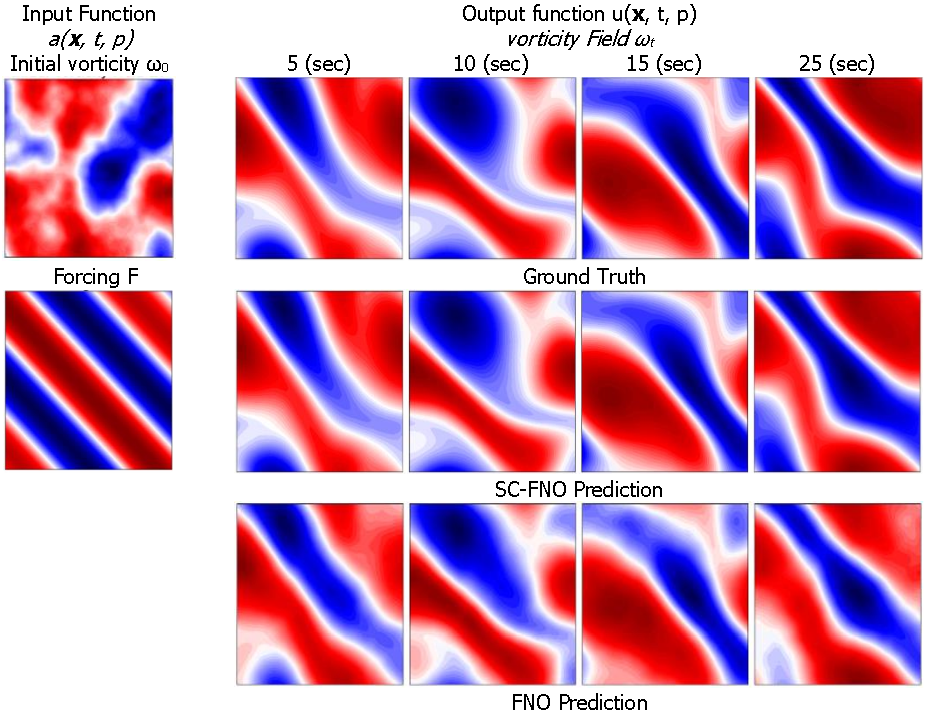
\includegraphics[width=0.8\textwidth, trim={0 0 0 0}, clip]{Figuers/PDE2_sample_prediction.pdf} % update filename if needed
%     \caption{\textbf{PDE2 Sample Prediction.}  
%     Representative forward prediction for PDE2 showing ground truth, SC-FNO, and FNO across selected time snapshots.  
%     SC-FNO maintains close agreement with the ground truth, while FNO exhibits dissipative drift and smeared structures over time.}
%     \label{fig:PDE2_sample_pred}
% \end{figure}



% Table for performances of models for inverse prediction of PDE2 without STD (rounded)
\begin{table}[ht!]
\centering
\caption{\scriptsize\textbf{Comparison of Error Metrics Across Models Trained with Different Sample Sizes (Inverse) PDE2}}
\label{tab:pde2_inverse_nostd}
\scriptsize
\setlength{\tabcolsep}{3pt}
\begin{tabular}{lcccccccc}
\hline
\textbf{Model} & \multicolumn{2}{c}{\textbf{1000 Samples}} & \multicolumn{2}{c}{\textbf{500 Samples}} & \multicolumn{2}{c}{\textbf{200 Samples}} & \multicolumn{2}{c}{\textbf{100 Samples}} \\
 & \textbf{Rel. \(L^2\)} & \textbf{MAE} & \textbf{Rel. \(L^2\)} & \textbf{MAE} & \textbf{Rel. \(L^2\)} & \textbf{MAE} & \textbf{Rel. \(L^2\)} & \textbf{MAE} \\
\hline
FNO        & \(4.7 \times 10^{-1}\) & \(5.0 \times 10^{-2}\) & \(6.7 \times 10^{-1}\) & \(7.2 \times 10^{-2}\) & \(9.6 \times 10^{-1}\) & \(1.0 \times 10^{-1}\) & \(1.4 \times 10^{0}\) & \(1.4 \times 10^{-1}\) \\
WNO        & \(5.6 \times 10^{-1}\) & \(5.9 \times 10^{-2}\) & \(7.9 \times 10^{-1}\) & \(8.4 \times 10^{-2}\) & \(1.1 \times 10^{0}\) & \(1.2 \times 10^{-1}\) & \(1.6 \times 10^{0}\) & \(1.7 \times 10^{-1}\) \\
DeepONet   & \(5.8 \times 10^{-1}\) & \(6.1 \times 10^{-2}\) & \(8.0 \times 10^{-1}\) & \(8.7 \times 10^{-2}\) & \(1.2 \times 10^{0}\) & \(1.2 \times 10^{-1}\) & \(1.6 \times 10^{0}\) & \(1.7 \times 10^{-1}\) \\
SC-FNO     & \(\mathbf{6.1 \times 10^{-2}}\) & \(\mathbf{5.2 \times 10^{-3}}\) & \(\mathbf{6.8 \times 10^{-2}}\) & \(\mathbf{5.8 \times 10^{-3}}\) & \(\mathbf{8.0 \times 10^{-2}}\) & \(\mathbf{6.8 \times 10^{-3}}\) & \(\mathbf{9.6 \times 10^{-2}}\) & \(\mathbf{8.2 \times 10^{-3}}\) \\
SC-WNO     & \(6.8 \times 10^{-2}\) & \(5.8 \times 10^{-3}\) & \(7.6 \times 10^{-2}\) & \(6.5 \times 10^{-3}\) & \(9.0 \times 10^{-2}\) & \(7.6 \times 10^{-3}\) & \(1.1 \times 10^{-1}\) & \(9.2 \times 10^{-3}\) \\
SC-DeepONet& \(8.3 \times 10^{-2}\) & \(7.0 \times 10^{-3}\) & \(9.3 \times 10^{-2}\) & \(7.9 \times 10^{-3}\) & \(1.1 \times 10^{-1}\) & \(9.3 \times 10^{-3}\) & \(1.3 \times 10^{-1}\) & \(1.1 \times 10^{-2}\) \\
\hline
\end{tabular}
\end{table}






% \begin{figure}[ht!]
%     \centering
%     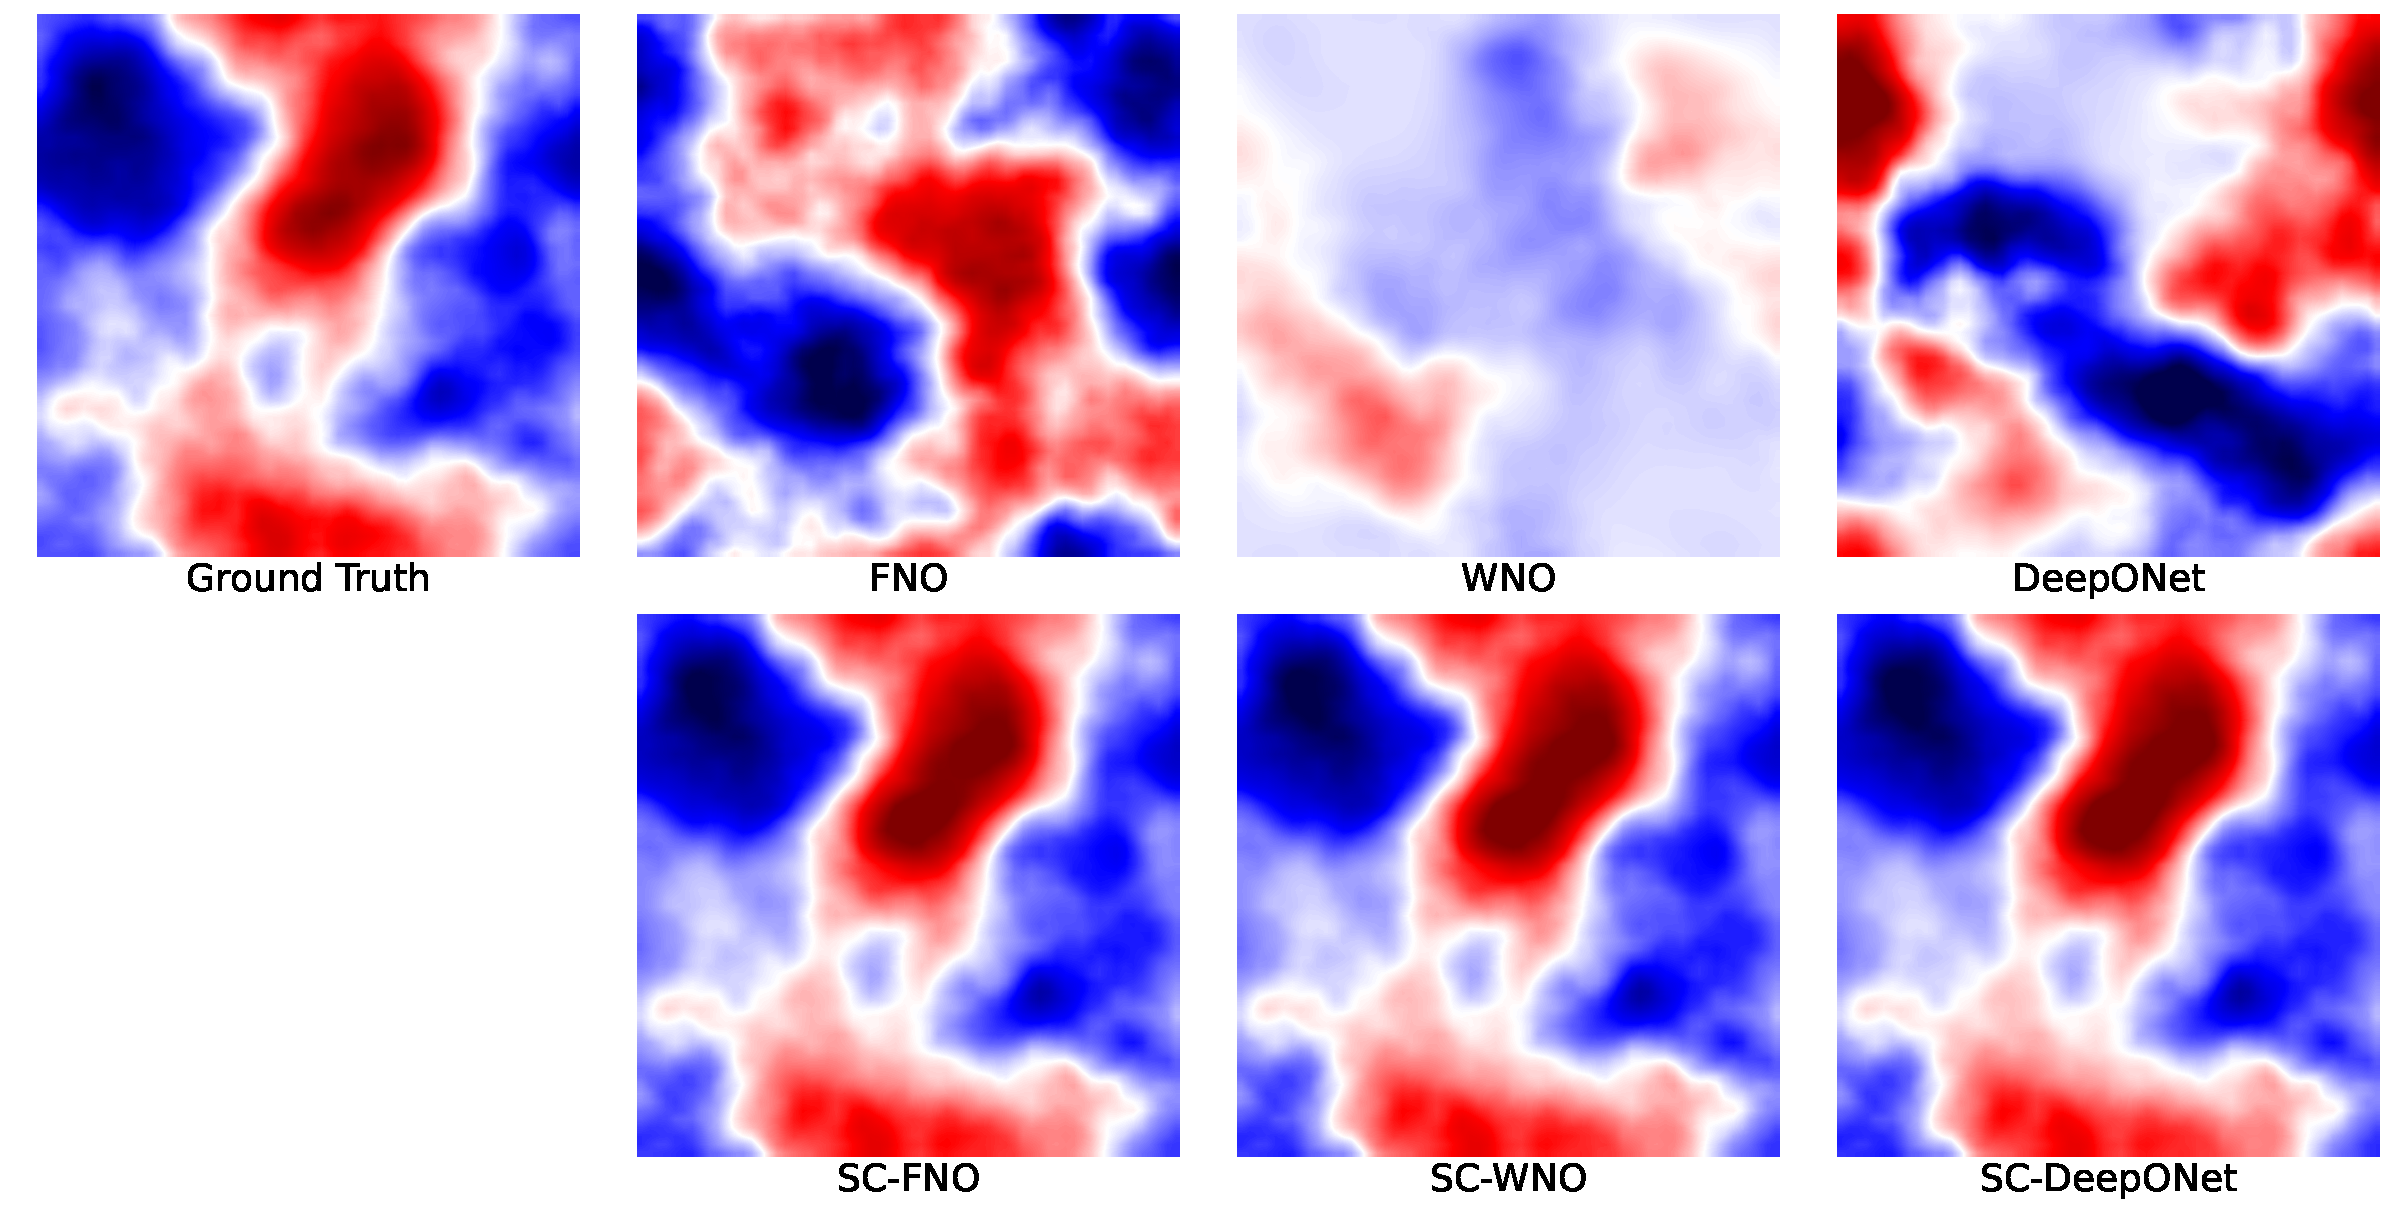
\includegraphics[width=0.8\textwidth]{Figuers/vorticity_reconstruction_clean_sample_5.pdf}
%     \caption{\textbf{Inversion of the Initial Vorticity Field for PDE2 (all models trained using 1000 samples).}
%     Comparison of the true initial vorticity field $\omega_0$ (top-left) with the inferred fields produced by FNO, WNO, DeepONet, and their sensitivity-constrained counterparts (SC-FNO, SC-WNO, SC-DeepONet). 
%     }
%     \label{fig:PDE2_w0_inversion}
% \end{figure}



\begin{figure}[ht!]
    \centering
    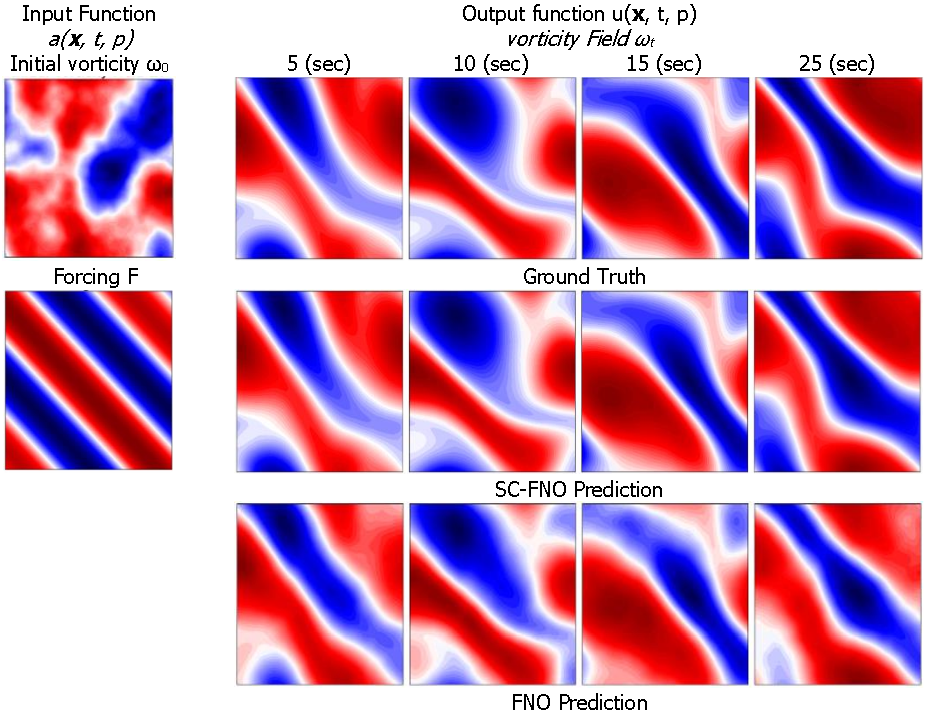
\includegraphics[width=0.8\textwidth, trim={0 0 0 0}, clip]{Figuers/PDE2_sample_prediction.pdf} % update filename if needed
    \caption{\scriptsize\textbf{PDE2 Sample Prediction.}  
    Representative forward predictions for PDE2 comparing the ground truth, SC-FNO, and FNO, trained on 200 samples, at selected time snapshots. SC-FNO maintains close agreement with the ground truth, while FNO exhibits dissipative drift and progressively smeared structures over time.}
    \label{fig:PDE2_sample_pred}
\end{figure}


\begin{figure}[ht!]
    \centering
    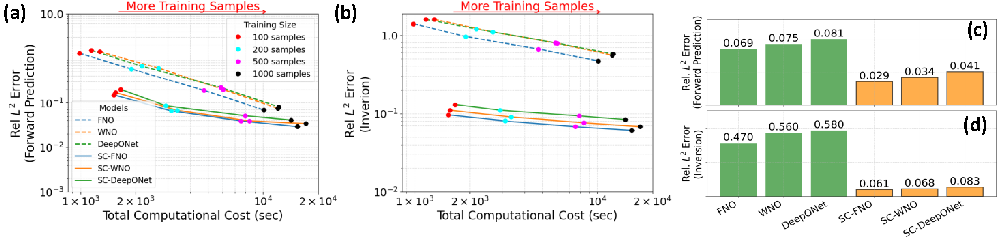
\includegraphics[width=0.98\textwidth, trim={0 0 0 0}, clip]{Figuers/PDE2_summeries.pdf}
    \caption{\scriptsize\textbf{Accuracy–computation trade-off for
    Turbulent Navier--Stokes with Spalart--Allmaras model (PDE2).}
    Sensitivity constraints achieve substantially lower errors for the same
    computational budget as training samples increase.
    (a) Relative $L^2$ error for forward prediction versus total computation time.
    (b) Relative $L^2$ error for inversion (reconstruction of $\omega$) versus total computation time.
    (c) Relative $L^2$ error for forward prediction at 1000 training samples.
    (d) Relative $L^2$ error for inversion at 1000 training samples.}
    \label{fig:PDE2_summerised}   
    \end{figure}



\begin{figure}[ht!]
    \centering
    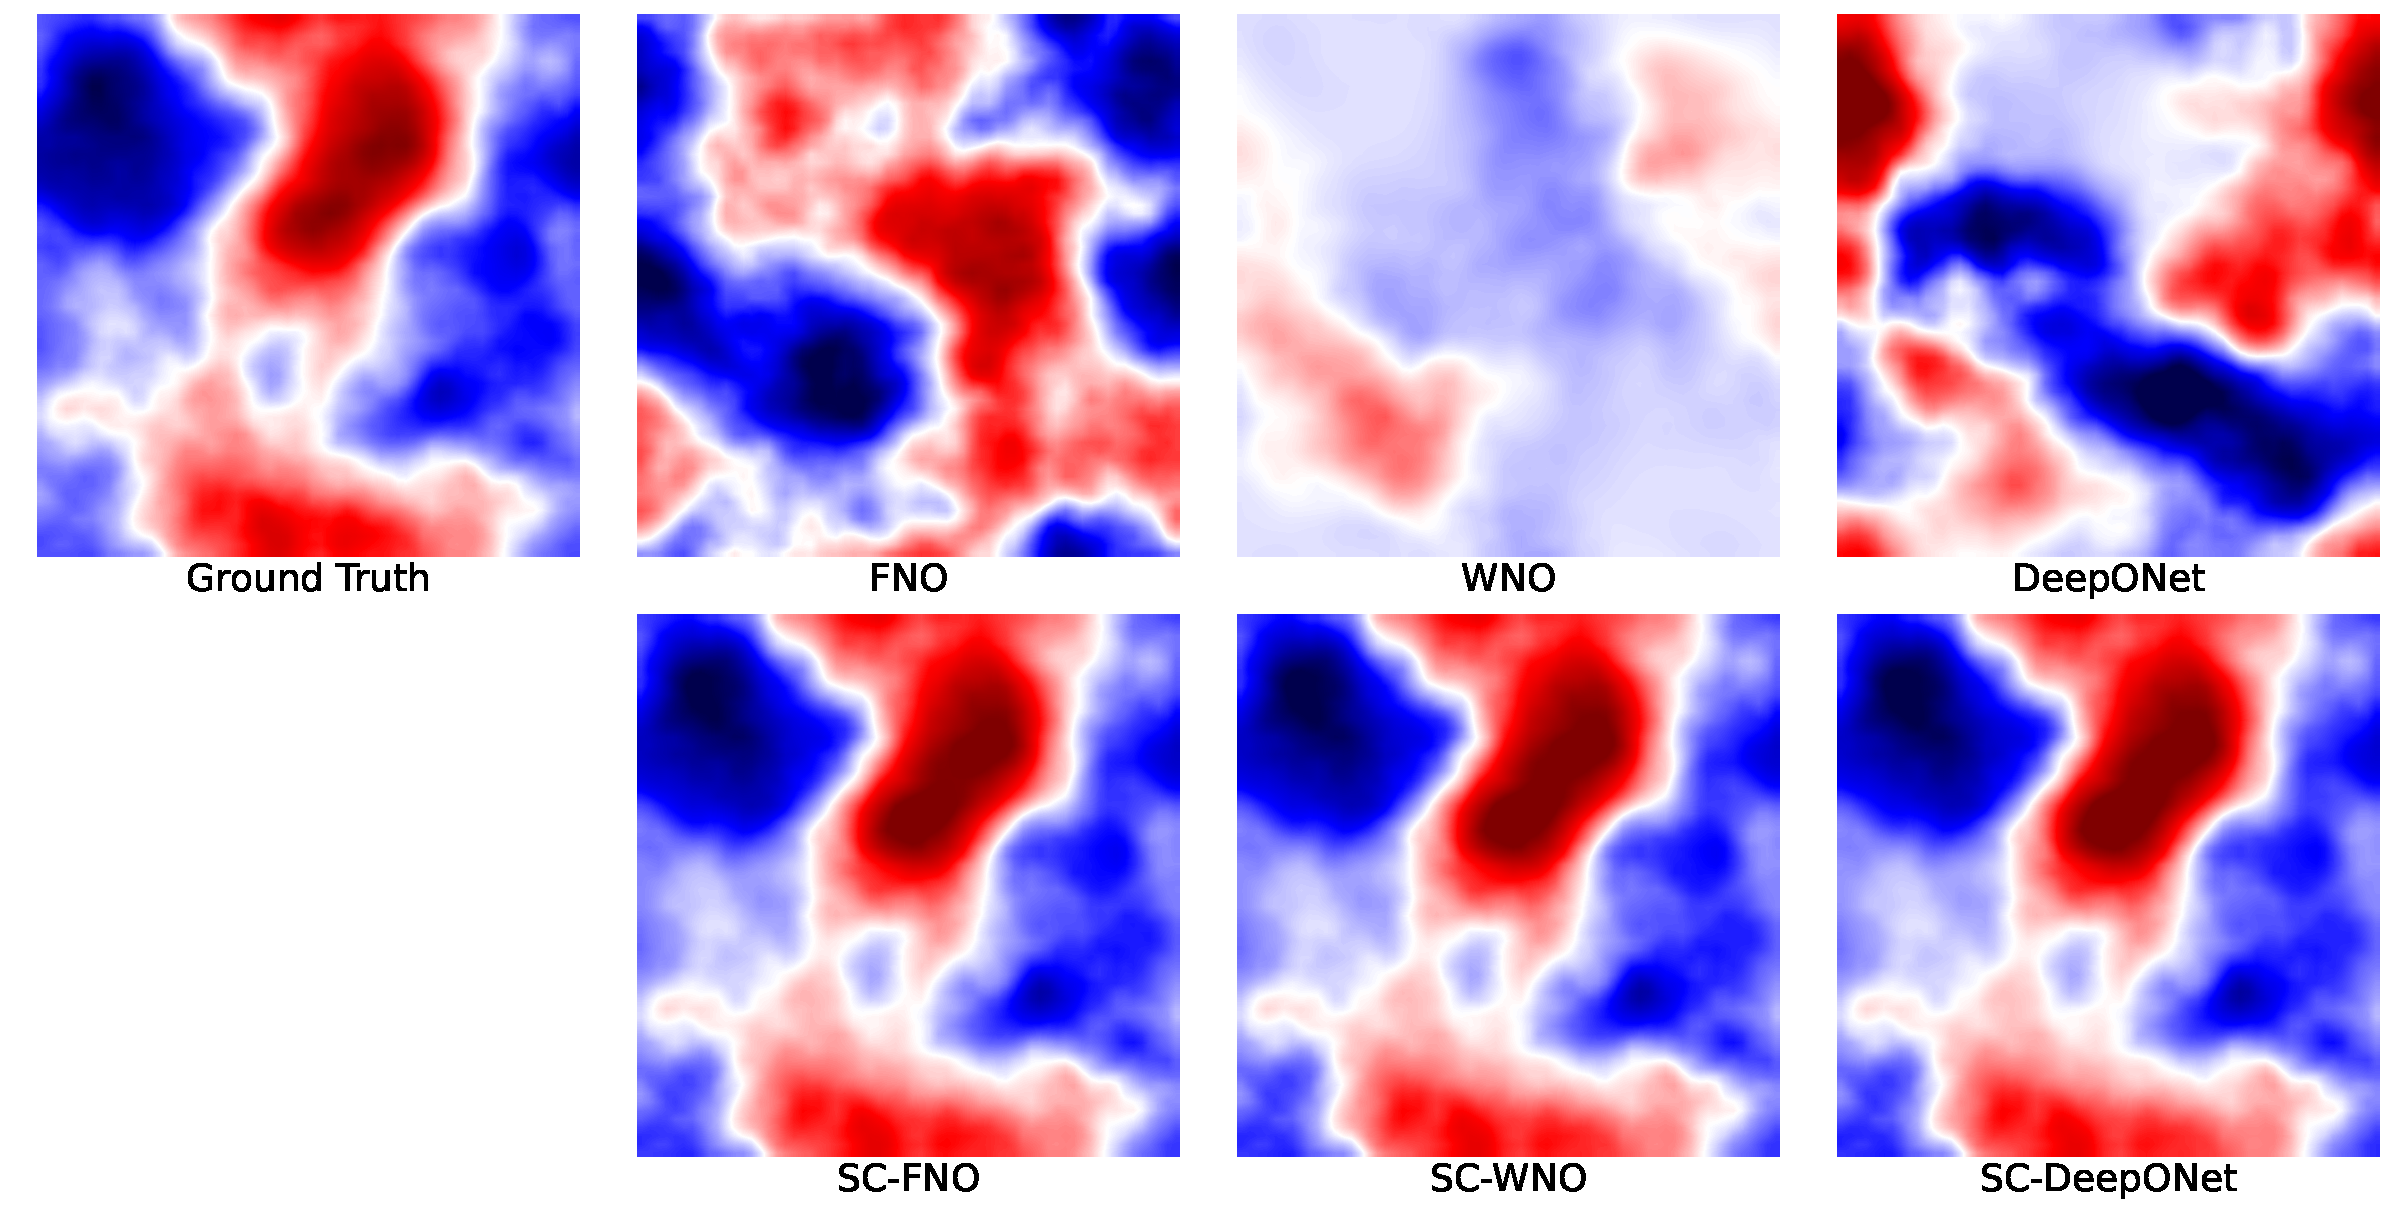
\includegraphics[width=0.8\textwidth]{Figuers/vorticity_reconstruction_clean_sample_5.pdf}
    \caption{\scriptsize\textbf{Inversion of the Initial Vorticity Field for PDE2 (all models trained using 200 samples).}
    Comparison of the true initial vorticity field $\omega_0$ (top-left) with the inferred fields produced by FNO, WNO, DeepONet, and their sensitivity-constrained counterparts (SC-FNO, SC-WNO, SC-DeepONet). 
    }
    \label{fig:PDE2_w0_inversion}
\end{figure}
